\section{Prüfverzahnung kst-E und Prüfräder}
\label{sec:pruefverzahnung}

Die Laufversuche und die Berechnungen dieser Arbeit beziehen sich auf die Prüfverzahnung kst-E der FZG, eine geradverzahnte Stahl-Kunststoff-Paarung mit dem Normalmodul $m_{\mathrm{n}} = 1$\,mm. Sie ist für den Verspannungsprüfstand mit dem Achsabstand $a_{\mathrm{w}} = 52$\,mm ausgelegt (\secref{sec:pruefstand}). Das Stahlritzel mit $z_{\mathrm{1}} = 51$ Zähnen treibt das Kunststoffrad mit $z_{\mathrm{2}} = 52$ Zähnen. Die Benennung lehnt sich an frühere Prüfverzahnungen des Lehrstuhls an \cite[S.~42 und 46]{Fie23}. Als Nenngeometrie dient der STplus-Fall kst-E, dessen Ergebnisliste (STplus 11.1F, 14.02.2025) am Lehrstuhl als Referenz dieser Paarung geführt wird. In \tabref{tab:geometrie_kste} stehen die Werte für Ritzel und Rad nebeneinander, wie sie die Geometriekette dieser Arbeit aus den Eingaben des Falls ausgibt (\secref{sec:werkzeugkette}). Die Bezeichnungen folgen DIN ISO 21771 \cite{DINISO21771}. Aus den Profilverschiebungsfaktoren $0{,}2034$ und $0{,}3143$ ergeben sich ein Betriebseingriffswinkel von $21{,}463$° und eine Profilüberdeckung von $1{,}154$. \figref{fig:stirnschnitt_kste} zeigt den Stirnschnitt der Paarung in der Stellung C mit den Kreisen der Tabelle, der Eingriffslinie und den Normpunkten A bis E.

\begin{figure}[htbp]
    \centering
    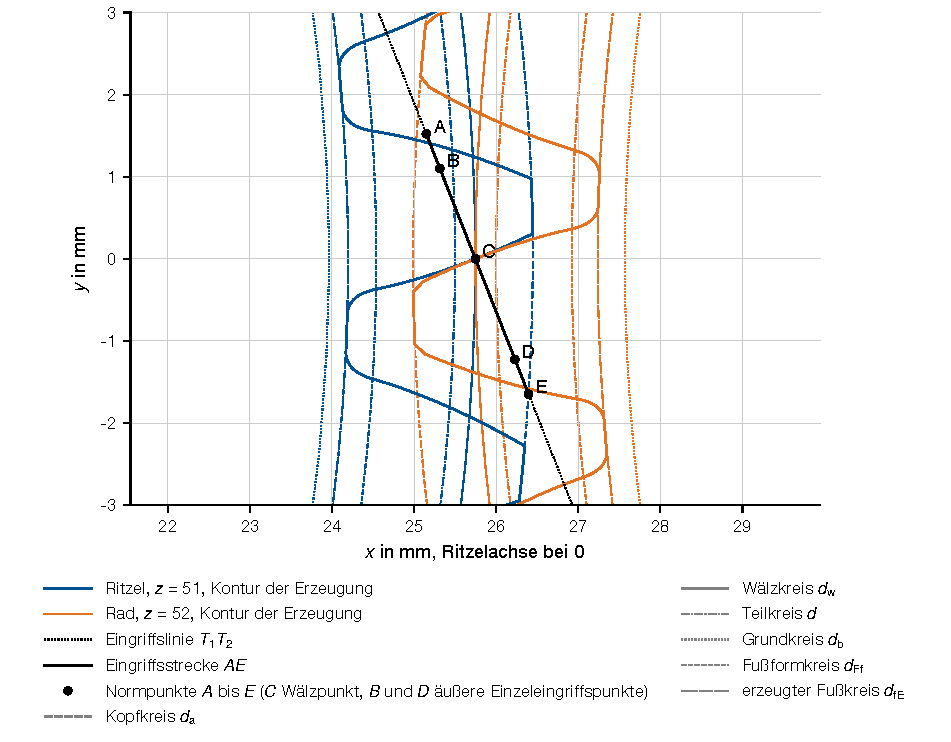
\includegraphics[width=0.9\textwidth]{kap3/stirnschnitt_kste}
    \caption{Stirnschnitt der Prüfverzahnung kst-E in der Stellung C: Konturen der Erzeugung, Kreise der Geometrietabelle, Eingriffslinie und Eingriffsstrecke mit den Normpunkten A bis E (das Ritzel treibt im Uhrzeigersinn, die rechten Flanken arbeiten).}
    \label{fig:stirnschnitt_kste}
\end{figure}

\begin{table}[htbp]
    \caption{Nenngeometrie der Prüfverzahnung kst-E nach dem STplus-Fall, ausgegeben durch die Geometriekette dieser Arbeit, und Werkstoffe nach den Zeichnungen.}
    \label{tab:geometrie_kste}
    \centering
    \begin{tabular}{llcc}
        Größe                               & Zeichen                              & Ritzel                         & Rad        \\
        \hline
        Zähnezahl                           & $z$                                  & $51$                           & $52$       \\
        Normalmodul in mm                   & $m_{\mathrm{n}}$                     & \multicolumn{2}{c}{$1{,}0$}                 \\
        Normaleingriffswinkel in °          & $\alpha_{\mathrm{n}}$                & \multicolumn{2}{c}{$20{,}000$}              \\
        Schrägungswinkel in °               & $\beta$                              & \multicolumn{2}{c}{$0$}                     \\
        Achsabstand in mm                   & $a_{\mathrm{w}}$                     & \multicolumn{2}{c}{$52{,}000$}              \\
        Profilverschiebungsfaktor           & $x$                                  & $0{,}2034$                     & $0{,}3143$ \\
        Zahnbreite in mm                    & $b$                                  & $17$                           & $15$       \\
        Teilkreisdurchmesser in mm          & $d$                                  & $51{,}000$                     & $52{,}000$ \\
        Grundkreisdurchmesser in mm         & $d_{\mathrm{b}}$                     & $47{,}924$                     & $48{,}864$ \\
        Wälzkreisdurchmesser in mm          & $d_{\mathrm{w}}$                     & $51{,}495$                     & $52{,}505$ \\
        Kopfkreisdurchmesser in mm          & $d_{\mathrm{a}}$                     & $52{,}894$                     & $54{,}022$ \\
        Fußformkreisdurchmesser in mm       & $d_{\mathrm{Ff}}$                    & $49{,}081$                     & $50{,}157$ \\
        erzeugter Fußkreisdurchmesser in mm & $d_{\mathrm{fE}}$                    & $48{,}394$                     & $49{,}524$ \\
        Kopfhöhenfaktor des Werkzeugs       & $h_{\mathrm{aP0}}/m_{\mathrm{n}}$    & $1{,}10$                       & $1{,}25$   \\
        Kopfrundungsfaktor des Werkzeugs    & $\rho_{\mathrm{aP0}}/m_{\mathrm{n}}$ & $0{,}20$                       & $0{,}20$   \\
        Fußformhöhenfaktor des Werkzeugs    & $h_{\mathrm{FfP0}}/m_{\mathrm{n}}$   & $1{,}30$                       & $0{,}8456$ \\
        Erzeugungsprofilverschiebungsfaktor & $x_{\mathrm{E}}$                     & $-0{,}203$                     & $0{,}012$  \\
        Zahnweite über $k = 6$ Zähne in mm  & $W_{\mathrm{k}}$                     & $17{,}090$                     & $17{,}180$ \\
        Zahnweitenabmaß in mm               &                                      & $-0{,}278$                     & $-0{,}207$ \\
        Betriebseingriffswinkel in °        & $\alpha_{\mathrm{wt}}$               & \multicolumn{2}{c}{$21{,}463$}              \\
        Profilüberdeckung                   & $\varepsilon_{\alpha}$               & \multicolumn{2}{c}{$1{,}154$}               \\
        Werkstoff nach Zeichnung            &                                      & 20MnCr5                        & PA46-GF30  \\
    \end{tabular}
\end{table}

Beide Räder sind im STplus-Fall über zahnstangenförmige Bezugsprofile erzeugt. Das Werkzeugprofil des Ritzels trägt eine Kopfhöhe von $1{,}10\,m_{\mathrm{n}}$ und einen Kopfrundungsradius von $0{,}20\,m_{\mathrm{n}}$. Die Zeichnung von 2022 schreibt dazu Profilschleifen vor. Für das Rad legt die Zeichnung die Zahnform über das Bezugsprofil eines Wälzfräsers mit $h_{\mathrm{aP0}} = 1{,}25$\,mm und $\rho_{\mathrm{aP0}} = 0{,}20$\,mm fest. Das Rad wird spritzgegossen, die Flanken bleiben ohne Nachbearbeitung. Die Fußrundung beider Räder ist die Trochoide der abgerundeten Werkzeugkopfkante zwischen dem Fußformkreis und dem erzeugten Fußkreis, am Rad also zwischen $50{,}157$\,mm und $49{,}524$\,mm. An der $30$°-Tangente weist die Ergebnisliste für das Rad einen bezogenen Fußrundungsradius von $0{,}38$ und eine Fußdickensehne von $2{,}197$\,mm aus, für das Ritzel $0{,}40$ und $2{,}068$\,mm. Die Kontur der Geometriekette dieser Arbeit gibt für das Rad dieselben Werte wieder (\figref{fig:zahnkontur_kste}). Am Kopf des Rades rechnet STplus mit einem Kantenbruch unter $45$° und einem Radialbetrag von $0{,}117$\,mm, während die Zeichnung eine Kopfrundung mit dem Radius $0{,}2$\,mm vorsieht. Mit den Zahnweitenabmaßen der Tabelle ergeben sich Zahnweiten von $16{,}812$\,mm am Ritzel und $16{,}973$\,mm am Rad. Die Zeichnungen schreiben als Fertigmaß $16{,}822$\,mm mit dem Abmaß $-0{,}021$\,mm und $17{,}002$\,mm mit dem Abmaß $-0{,}059$\,mm vor.

%\Note{PH: Abgleich aller Zeichnungsfelder gegen den STplus-Fall (M7a) steht aus; Tabelle der Unterschiede nachtragen.}

\begin{figure}[htbp]
    \centering
    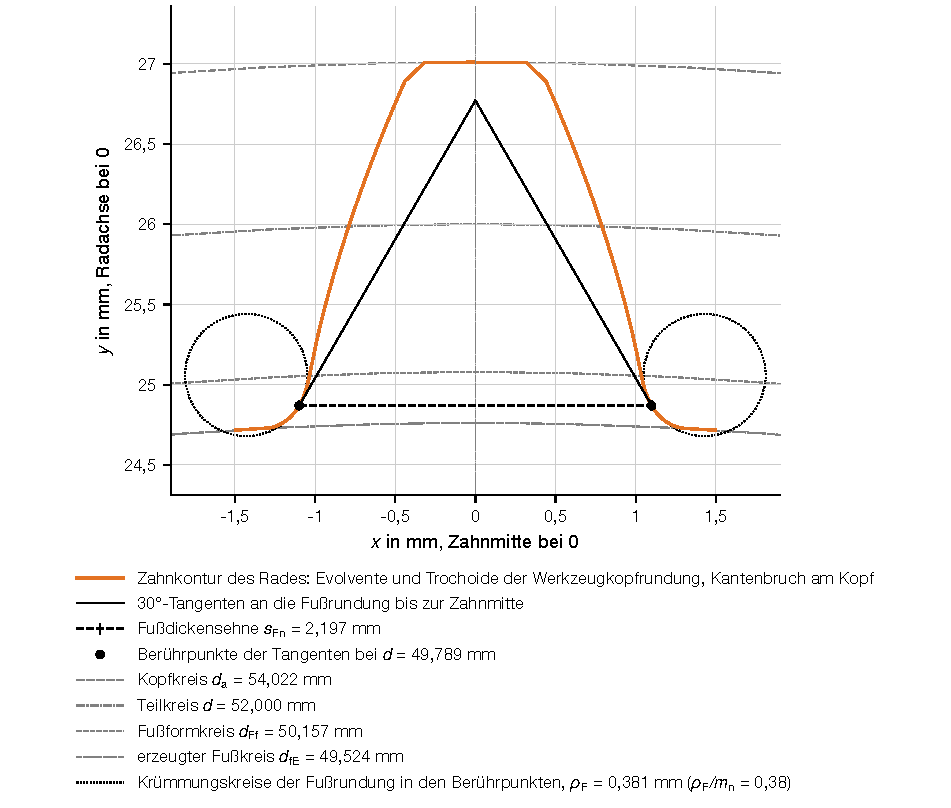
\includegraphics[width=0.85\textwidth]{kap3/zahnkontur_kste}
    \caption{Zahn des Rades kst-E im Stirnschnitt: Evolvente, Trochoide der Werkzeugkopfrundung und Kantenbruch, die Kreise der Erzeugung, die $30$°-Tangenten mit Fußdickensehne und Krümmungsradius aus der Kontur der Geometriekette.}
    \label{fig:zahnkontur_kste}
\end{figure}

Das Ritzel besteht nach beiden Zeichnungsständen aus dem Einsatzstahl 20MnCr5, der gasaufgekohlt und in Öl abgeschreckt wird. Gefordert sind eine Randhärte von $670$ + $100$\,HV\,1 und eine Einhärtetiefe von $0{,}3$ + $0{,}1$\,mm bei der Grenzhärte $550$\,HV\,1. Die Kernfestigkeit liegt zwischen $900$\,N/mm$^{2}$ und $1300$\,N/mm$^{2}$. Die Zeichnung von 2022 verlangt profilgeschliffene Flanken mit $R_{\mathrm{a}}$ von $0{,}20$\,\textmu m bis $0{,}25$\,\textmu m und eine Qualität besser als 6 nach DIN 3961 bis 3967. Dazu kommt eine lineare Kopfrücknahme $C_{\mathrm{a}} = 25$\,\textmu m ab dem Durchmesser $51{,}946$\,mm. Der Zeichnungsstand von 2025 beschreibt nur die Vorverzahnung mit einem Protuberanzfräser (Kopfhöhe $1{,}34\,m_{\mathrm{n}}$, Kopfrundung $0{,}25\,m_{\mathrm{n}}$) sowie geschliffene Bohrung und Planflächen. Die Endbearbeitung steht nicht auf der Zeichnung, weil sie in der Werkstatt des Lehrstuhls erfolgt. Dort werden die Flanken nachgeschliffen und die Kopfrücknahme eingebracht. In der Verzahnungsmessung zeigen die Prüfstandsritzel deshalb die Kopfrücknahme und die Zahnweite der Zeichnung von 2022 (\secref{sec:pruefraeder_vorher}). Im FE-Modell wird das Ritzel als Modellwahl ohne Kopfrücknahme nach der Nenngeometrie des STplus-Falls abgebildet (\secref{sec:fe_modell}). Im STplus-Fall selbst ist das Ritzel mit der Werkstoffkarte 16MnCr5 und das Rad mit einer Karte für PA66 belegt. Beide Karten dienen allein der Geometrie. Die Werkstoffdaten der Berechnung stammen aus den Zugversuchen in \secref{sec:fe_modell}.

Das Rad wird aus dem glasfaserverstärkten Polyamid 46 PA46-GF30 (Stanyl TW200F6 von Envalior) auf einen Stahleinleger gespritzt. Die Zeichnung des Rades nennt als Fertigung Spritzgießen und als Verzahnungsqualität Q10 nach DIN ISO 1328-1:2018-03. Die Bohrung 20 G6 mit der Passfedernut 6 J8 liegt im Einleger. Der Kunststoff ist in den Nuten des Einlegers eingespritzt und so gegen axiales Verschieben gesichert, das Rad sitzt über eine Passfeder auf der Welle \cite[S.~47]{Fie23}. Die Räder dieser Arbeit tragen dieselben Einleger aus 16MnCr5 wie die Räder der Laufversuche 2023. Der Kunststoffkörper beginnt beim Durchmesser $33$\,mm, die Nabe reicht in voller Breite bis zum Radius $19{,}107$\,mm. Von beiden Stirnseiten ist je eine $5{,}5$\,mm tiefe Tasche bis zum Radius $22{,}168$\,mm ausgespart. Ihre Wände stehen unter $93$° zur Stirnseite, so dass die Tasche mit der Tiefe schmaler wird. Drei der Ecken tragen den Radius $0{,}5$\,mm. Zwischen den Taschengründen bleibt ein Steg von $4$\,mm Dicke, außen trägt die Felge die Verzahnung über die volle Zahnbreite von $15$\,mm (\figref{fig:netz_koerper} in \secref{sec:fe_modell}). Für das Rad liegt ein Zeichnungsstand vor (Ausgabe 28.02.2022), für das Ritzel die Stände vom 08.06.2022 und vom 02.04.2025.

% gestrichen (TK kap3_6:87): Bild radkoerper_kste; der Radkörper steht nur noch in 3.6 als Bild netz_koerper, dort mit der z-Achse horizontal.

% TK erledigt (Bild hier gestrichen; netz_koerper in 3.6 mit z horizontal und weniger Maßen neu gezeichnet): Bitte die z-Achse auf die horizontale Ordinate, dann kann man sich den Zahnradkörper im Werschnitt besser vorstellen. Bitte weniger Radius und rundungsbemaßungen, die sind über die ordinaten ersichtlich, dann ist die Zeichnung auch aufgeräumter und überlappt nicht so stark. Entsprechend die Zeichnung überarbeiten.

Für die Laufversuche und die Messungen stehen 36 Räder und 8 Ritzel mit fünfstelligen Teilenummern der Stückliste zur Verfügung (\tabref{tab:teilegruppen_kste}). Zehn Räder bilden die Kerngruppe der eigenen Laufversuche auf dem Prüfstand KV3. Darunter diente 97351 dem Vorversuch zur Temperatur, und 97361 wurde nicht mehr gefahren, weil der Prüfstand nach dem Ausfall des Drehzahlsensors gewartet wird. Alle übrigen 26 vermessenen Räder bilden die Gruppe der Fertigungsstreuung. Dazu zählt das Rad 97364, das als zweites Rad der Stufe $8$\,Nm lief und von einer studentischen Hilfskraft vermessen wurde. Sieben Ritzel der Nummern 95911 bis 95920 gehören zur Serie, aus der das Prüfstandsritzel stammt. Sie wurden im Oktober 2025 vermessen. Das Ritzel 86481 ist ein älteres Stück mit einem Konturscan aus dem Jahr 2023. Sein Fußkreis liegt $0{,}17$\,mm unter dem der Serie, es ist anders geschnitten und dient nicht als Referenz. Der Zahn 1 ist auf den Teilen markiert und wird von Messmaschine, Konturscan und Prüfstand gleich gezählt. Die Laststufen je Teil stammen aus der Versuchsdatei des Prüfstands (\secref{sec:pruefstand}). Der Messumfang je Gruppe folgt in \secref{sec:dokumentation_pruefraeder}.

% TK erledigt (97351 Vorversuch, 97361 nicht gefahren, 97364 bei 8 Nm): Bitte den Absatz auf aktuellen Stand bringen

\begin{table}[htbp]
    \caption{Teilegruppen der Prüfräder kst-E nach den Teilenummern der Stückliste.}
    \label{tab:teilegruppen_kste}
    \centering
    \small
    \begin{tabular}{L{3.4cm}L{5.6cm}lL{4.4cm}}
        Gruppe                      & Teilenummern                                                         & Anzahl & Bemerkung                                                                          \\
        \hline
        Kernräder der Laufversuche  & 97340, 97345, 97346, 97350, 97351, 97355, 97360, 97361, 97365, 97366 & 10     & 97351 Vorversuch, 97361 ($8$\,Nm) aufgrund Prüfstandswartung noch nicht untersucht \\
        Fertigungsstreuung          & 97341 bis 97375 ohne Kernräder                                       & 26     & einschließlich 97364                                                               \\
        Zusatzversuch               & 97364                                                                & 1      & $8$\,Nm, zweites Rad der Stufe, zählt zur Streuung                                 \\
        Serie des Prüfstandsritzels & 95911, 95912, 95915, 95917, 95918, 95919, 95920                      & 7      & Verzahnungsmessung Oktober 2025                                                    \\
        älteres Ritzel              & 86481                                                                & 1      & Konturscan 2023                                                                    \\
    \end{tabular}
\end{table}

% Bildwunsch: Stirnschnitt der Paarung mit Bezeichnungen (Teil-, Grund-, Wälz-, Kopf-, Fußform- und Fußkreis,
%   Eingriffslinie, Normpunkte A bis E), Label fig:stirnschnitt_kste (eigene Zeichnung aus der Geometriekette, T5).
% Bildwunsch: Zahnkontur des Rades mit Fußrundung (Trochoide), Fußformkreis und 30-Grad-Tangente, Label
%   fig:zahnkontur_kste (T5-Skript).
% Bildwunsch: Radkörperschnitt (Meridianhalbschnitt durch die Zahnmitte: Einleger, Nabe, Taschen, Steg, Felge, Maße),
%   Label fig:radkoerper_kste (eigene Zeichnung T5 nach 90_CAD/Schnitt_Symmetrie_Zahnradkoerper_mit_Zahn.png).

% Herkunft:
% Absatz 1: Achsabstand 52 mm und Prüfstand: 00_gliederung.md Zeile 3.2; MA-0296.txt (pdftotext) Z. 1672 (PDF S. 52);
%   Benennung kst-E: MA-0296 Abschnitt 4.2, PDF S. 55 (gedruckt S. 42), Verweis auf [Rei22] PDF S. 59 (gedruckt S. 46);
%   Ritzel treibt: kst-E_eingabe.ste RAD_1_TREIBT; Referenzpaar "verified": scripts/oracle_cases.yaml Fall kst_e;
%   Ergebnisliste 11.0F vom 14.02.25: kst-E-ausgabe.sta Blatt 1; α_wt 21,463°, ε_α 1,154: gearcore-Ausgabe
%   (compute_generation_from_data) und .sta Blatt 6.
% Tabelle 1 (Zeile für Zeile): z, m_n, α_n, β, a, x, b, d_a, W_k, Abmaße: kst-E_eingabe.ste Zeilen 5 bis 17 und
%   .sta Blatt 6/7; d, d_b, d_w: gearcore-Ausgabe (reference, base, working pitch diameter) = .sta Blatt 6;
%   d_Ff 49,081/50,157 und d_fE 48,394/49,524: gearcore root_form_diameter_mm, generated_root_diameter_mm
%   (STplus druckt einfachgenau 50,158 und 49,523); Werkzeugfaktoren: .ste Blöcke WKZ_Profil_B_Ritzel/_Rad und
%   .sta Blatt 7/8 (h_FfP0* 1,300 für das Ritzel vom Programm belegt, gearcore root_form_height_factor 1.3);
%   x_E: gearcore −0,2032/0,0121, .sta Blatt 8 −0,2030/0,0117 (auf drei Stellen gleich);
%   α_wt, ε_α: s. o.; Werkstoff nach Zeichnung: 20220623/20250402 (20MnCr5), parts.yaml (PA46-GF30).
% Absatz 2: Bezugsprofile und Profilschleifen: .ste; Zeichnung Ritzel 20220623 (Flankenbearbeitung Profilschleifen,
%   haP0 1,10 mn, rhoaP0 0,20 mn); Zeichnung Rad 20220316 (Werkz.-Profil Wälzfräser, haP0 1,25 mm, rho_aP0 0,20 mm,
%   Spritzgegossen, keine Nachbearbeitung); Fußrundung Fußformkreis bis Fußkreis: gearcore-Werte s. Tabelle;
%   30-Grad-Tangente rho_F* 0,40/0,38, s_fn* 2,068/2,197: .sta Blatt 11; Kantenbruch 45° und h_K 0,117 mm: .sta Blatt 6
%   und 9; Kopfrundung r 0,2 mm: Zeichnung Rad 20220316; Zahnweiten 16,812/16,973 mm: ADR-117 Amendment 2026-10-12
%   Punkt 1 und 3 (architecture_decisions.md Z. 2086 und 2101); Fertigmaße: Zeichnung Ritzel 20220623 (16,822 −0,021),
%   Zeichnung Rad 20220316 (17,002 −0,059); M7a offen: implementation_roadmap.md Z. 129.
% Absatz 3: Werkstoff, Wärmebehandlung, Härte, Einhärtetiefe, Kernfestigkeit, Ra, Qualität, Kopfrücknahme 25 µm ab
%   51,946 mm: Zeichnung Ritzel 20220623; Protuberanzfräser 1,34 mn / 0,25 mn, Bohrungs- und Planflächenschleifen, kein
%   Zahnflankenschleifen: Zeichnung Ritzel 20250402; Endbearbeitung (Nachschleifen der Flanken und Kopfrücknahme) in
%   der Werkstatt des Lehrstuhls, nicht auf der Zeichnung: Angabe des Nutzers, Kommentar in dieser Datei 2026-10-17;
%   Prüfstandsritzel zeigen Rücknahme und Zahnweite 2022: ADR-116
%   Punkt 44 (architecture_decisions.md Z. 1536 bis 1539), ADR-118 Punkt 8 (Z. 2217 bis 2222); FE-Ritzel ohne
%   Rücknahme nach STplus-Nenngeometrie: ADR-116 Punkt 44 (Z. 1543 bis 1544, "base geometry stays"), .ste
%   OHNE_RUECKNAHME = ja;
%   Werkstoffkarten 16MnCr5 / PA66: .ste WERKSTOFF; Zugversuche als Werkstoffquelle: ADR-118 Kontext (Z. 2169 bis 2171).
% Absatz 4: PA46-GF30 Stanyl TW200F6 (Envalior): parts.yaml (material), ADR-119 Kontext (Z. 2701), sources.yaml
%   CAMPUS-StanylTW200F6:2024; Spritzgießen, Q10 DIN ISO 1328-1:2018-03, Bohrung 20 G6, Nut 6 J8, Stahleinleger:
%   Zeichnung Rad 20220316; Nuten des Einlegers, Passfeder, Einleger 16MnCr5 (Räder 2023): MA-0296 PDF S. 59/60
%   (gedruckt S. 46/47); Radkörpermaße (Bohrung 33 mm, Nabe r 19,107, Tasche 5,5 tief bis r 22,168, 93°, R 0,5,
%   Steg 4 mm, b 15): data/fe/body_sections.yaml und 80_output/fe/kst_e/frozen_mesh_20layers_bore33_pocket/README.md
%   Absatz 2; Zeichnungsstände: Ausgabedaten auf den drei Zeichnungen (28.02.2022, 08.06.2022, 02.04.2025).
% Absatz 5 und Tabelle 2: Gruppen, Teilenummern, Einlauf 97351, 97361 läuft (8 Nm), 97364 Zusatzversuch 12 Nm durch
%   Hilfskraft, Serie 95911 bis 95920 (GINA Oktober 2025), 86481 nur Konturscan 2023, Zahn 1 markiert:
%   data/measurement/parts.yaml (provenance.notes, groups, labels); Zählung 44 Teile = 10 + 26 + 7 + 1:
%   80_output/messungen/inventory/inventory.md Kopf und Zähltabellen, ADR-117 Consequences (Z. 1998 bis 1999);
%   86481 Fußkreis 0,17 mm unter der Serie, anders geschnitten, keine Referenz: ADR-117 Amendment 2026-10-12
%   Punkt 4 (Z. 2131 bis 2133); Laststufen aus der Prüfstandsdatei: parts.yaml provenance.notes.
% Nomenklatur: alpha_wt (Betriebseingriffswinkel), x_E (Erzeugungsprofilverschiebungsfaktor), h_FfP0
%   (Fußformhöhe des Werkzeug-Bezugsprofils) fehlen noch in Nomenklatur.tex; d_f der Zeichnungen wird im Text
%   nicht als Symbol verwendet, der erzeugte Fußkreis steht als d_fE.
